\chapter{Evaluatie bestaande representaties}

We beoordelen de bestaande representaties van de drie onderzochtte complexen en proberen hier vervolgens een algemene conclusie aan te verbinden. De beoordelingen zijn gebaseerd op een congnitive walkthrough en onderzoek naar de cognitive dimensions.


\section{Cognitive walkthrough}


\subsection{De methode} \label{sectie:cw_methode}

Om de methode van cognitive walkthrough toe te passen kiezen we een stakeholder en een taak van deze stakeholder. Dit zal een taak zijn die door veel stakeholders uitgevoerd kan worden. Bij deze taak sommen we mogelijke acties op die samen tot het volbrengen van de taak kunnen leiden.

Deze acties projecteren we vervolgens op de representatie. We kijken per actie of de gebruiker merkt dat deze mogelijk is, of de gebruiker bedenkt dat deze actie ook echt een juiste is, en of de gebruiker merkt dat het goed gaat nadat hij de actie uitgevoerd heeft.


\subsection{Toepassing} \label{sectie:cw_toepassing}

De cognitive walkthrough passen we toe op de bezoeker van een evenement (zie \ref{sectie:stkh_bzkr} voor deze stakeholder) met de taak het vinden van een toilet. Omdat deze taak erg algemeen is, is hij voor veel stakeholders relevant en dus erg geschikt voor de cognitive walkthrough. Voor de verschillende bestaande representaties gebruiken we deze zelfde stakeholder en taak om de cognitive walkthrough toe te passen.


\subsection{RAI Amsterdam}

We bespreken de volgende acties die nodig zijn om het doel te bereiken in de RAI met de huidige bewegwijzering:


\subsubsection{Huidige locatie bepalen}

In de RAI hangen in iedere ruimte en bij alle in- en uitgangen plattegronden van het complex. Op een plattegrond wordt met een geel handje aangegeven waar je je op dat moment bevindt. Dit werkt met de bewegwijzering die de RAI hanteert vrij goed. Daarbij zijn de borden situatie-gericht, zodat je je ook meteen kunt ori\"enteren in welke richting je kijkt en je dus beter kunt bepalen waar je heen moet lopen.

Wat niet wordt aangegeven is op welke verdieping je je bevindt. Dit zorgt voor verwarring in bepaalde situaties, wat in het ergste geval zelfs kan betekenen dat je niet kunt vinden wat je zoekt.

In de hallen hangen in het midden aan het plafond grote vanen met daarop het halnummer. Binnen een hal kun je dus altijd gemakkelijk zien om welke hal het gaat.


\subsubsection{Locatie van doel bepalen}

Op de plattegrond wordt met iconen gewerkt. Voor toiletten worden een mannetje en vrouwtje die naast elkaar staan gebruikt. Indien er ook een invalide-toilet aanwezig is, wordt dat aangegeven met een mannetje in een rolstoel. Deze iconen staan duidelijk aangegeven op de plattegrond, dus het is makkelijk om te bepalen waar een toilet is.


\subsubsection{Route naar doel bepalen}

Omdat je gemakkelijk je huidige locatie en de locatie van je doel kunt bepalen, is het niet moeilijk een route uit te stippelen. Sowieso is het in de RAI niet echt moeilijk een toilet te vinden, omdat er vrij veel zijn. Hierdoor hoef je altijd maar weinig hindernissen te nemen (zoals in- en/of uitgangen vinden).

Maar hier komt wel weer het probleem naar voren van het slecht aangeven op welke verdieping je je bevindt (en je doel). Je kunt dus vrij lastig inschatten of je route langs een trap of lift moet lopen.


\subsubsection{Bepalen of het doel bereikt is}

Op de deuren van de WC's hangen bordjes met een mannetje, vrouwtje, of rolstoel erop, die aangeven voor welke groep mensen het toilet bedoeld is. Aan de hand van die bordjes kun je ook snel zien dat je je doel bereikt hebt. Ook bij de alle ingangen van de hallen zijn bordjes met het halnummer aanwezig.


\subsection{AHOY Rotterdam}

We bespreken de volgende acties die nodig zijn om het doel te bereiken in AHOY met de huidige bewegwijzering:


\subsubsection{Huidige locatie bepalen}

In de hallen van AHOY zijn op de wanden halnummers aangebracht, binnen een hal is het dus niet moeilijk uit te zoeken waar je bent. De hallen liggen rond een centraal gebouw, dat, afgezien van grote evenementen in het Sportpaleis, de ingang biedt voor alle evenementen. Verder zijn er geen gebouwen, dus wanneer je je niet in een hal bevindt is het ook niet moeilijk meer.

In AHOY zijn geen plattegronden te vinden, ook niet bij de ingangen. Dit is echter geen groot gemis, door de veel eenvoudiger opbouw van het complex dan bij de RAI Amsterdam het geval is.


\subsubsection{Locatie van doel bepalen}

Door het ontbreken van plattegronden kun je niet direct zien waar je doel zich bevindt, tenzij het binnen je gezichtsveld ligt. Om je route te bepalen ben je dus afhankelijk van de richtingen die door de bewegwijzering worden aangegeven.


\subsubsection{Route naar doel bepalen}

Zoals hierboven naar voren kwam wordt je route bepaald door de bewegwijzering. Gelukkig geeft deze erg goed de richting aan van vrijwel alles. Wordt je doel niet aangegeven, dan loop je vanzelf naar de centrale hal waar de richting wel wordt aangegeven.

Op de borden wordt alles aangegeven met tekst en eventueel een icoon. Daarnaast wordt erbij vermeld op welke verdieping je moet zijn wanneer dit niet de begane grond is en of het bord je richting een roltrap of lift stuurt.

Wanneer je de locatie van een evenement zoekt wordt het nog gemakkelijker. Je hoeft geen halnummer of verdieping te weten, alles wordt aangegeven met de naam van het evenement. Er staan zuilen bij de ingang en roltrappen met daarop de namen van evenementen en de richting. Wederom wordt de etage erbij vermeld en staan er eventuele iconen voor roltrap of lift.


\subsubsection{Bepalen of doel bereikt is}

Bij alle faciliteiten zoals toilet, garderobe, parkeerautomaat en lift hangen bordjes met iconen en/of tekst. In het geval van de toiletten hangen er iconen van mannetjes, vrouwtjes en rolstoelen. Ook bij de ingangen van de hallen wordt het halnummer vermeld. In het geval van een evenement wordt ook de naam hiervan gebruikt.


\subsection{VU Academisch Ziekenhuis Amsterdam}

We bespreken de volgende acties die nodig zijn om het doel te bereiken in het VU Ziekenhuis met de huidige bewegwijzering:


\subsubsection{Huidige locatie bepalen}

In het VU ziekenhuis kom je als eerste bij een informatiebalie. Verder is er een algemeen becijferingssysteem voor alle kamers die eerst bestaat uit de verdieping waar je moet zijn dan de afdeling en dan het specifieke kamernummer. Het ziekenhuis is dan opgedeeld in de afdelingen A t/m D. In het hele ziekenhuis hangen allemaal borden met pijlen gericht naar de verschillende afdelingen met verder nog specifiekere borden, als je al op een afdeling bent, waar de verschillende kamers liggen (bijvoorbeeld de kamers 100-111). Er wordt hier verder niet met plattegronden gewerkt, wel is er een algemene plattegrond die alleen de afdelingen weergeeft. Specifieker is ook niet mogelijk vanwege de complexe structuur van het ziekenhuis. Verder heb je bij omleidingen nog gele blaadjes met richtingen voor als de normale route niet te gebruiken is, deze geven meteen de specifiekere locatie aan zoals eerder beschreven.


\subsubsection{Locatie van doel bepalen}

Om de locatie van het doel te bepalen ga je bij de ingang naar de informatiebalie. Hier geef je aan wat je doel is en zij vertellen dan waar je moet zijn, je krijgt dan dus de verdieping met de afdeling en het kamernummer. Verder nog kort een uitleg over welke richting je in ieder geval op moet.


\subsubsection{Route naar doel bepalen}

De route wordt deels bepaald door de begin richting en de korte uitleg die je bij de informatiebalie hebt gekregen. Verder zie je de borden naar welke afdeling je moet. Je gaat dan eerst naar de juiste afdeling waar je dan moet zijn (op iedere afdeling zijn liften om naar een andere verdieping te gaan). Vervolgens naar de juiste verdieping, daar volg je dan de specifiekere borden naar de juiste kamers waar je vervolgens het juiste nummer zoekt.


\subsubsection{Bepalen of doel bereikt is}

De vordering in je zoek actie merk je door dat je steeds specifiekere aanduidingen krijgt van je doel. Het is ook lastig om van te voren een route uit te stippelen als je het gebouw niet echt kent. Het enige dat van te voren te plannen is, is de informatie die je vraagt bij de informatiebalie bij de entree.


\section{Cognitive dimensions}

Verschillende cognitieve dimensies projecteren we op de bewegwijzering van de RAI Amsterdam, AHOY Rotterdam en het VU Academisch Ziekenhuis Amsterdam. We noemen de positieve en negatieve punten van de systemen.


\subsection{Belangrijkste dimensies} \label{sectie:cd_demensies}

We zullen de belangrijkste cognitieve dimensies hier opnoemen en kort uitleggen wat ermee bedoeld wordt:


\begin{itemize}

\item \emph{Viscosity}

De moeite die gedaan moet worden om (kleine) wijzigingen in het systeem aan te brengen.

\item \emph{Hidden dependencies}

Afhankelijkheden tussen delen van de representatie die niet direct zichtbaar zijn.

\item \emph{Premature commitment}

Het dwingen van de gebruiker tot een beslissing voor de juiste hoeveelheid informatie voor hem/haar beschikbaar is doordat de volgorde van acties vast ligt.

\item \emph{Abstractions}

Het groeperen van entiteiten om de viscositeit te verlagen of om de representatie beter aan te laten sluiten bij de gebruiker.

\item \emph{Secondary notation}

Informatie die aan de representatie toegevoegd wordt terwijl deze geen wezenlijk deel uitmaakt van het gerepresenteerde maar het bijvoorbeeld gemakkelijker maakt de representatie te interpreteren.

\item \emph{Visibility \& Juxtaposibility}

Visibility is het gemak waarmee onderdelen van de representatie te zien zijn. Juxtaposibility is het gemak waarmee deze onderdelen te vergelijken zijn.

\end{itemize}


\subsection{RAI Amsterdam} \label{sectie:cd_rai}

We bespreken de bewegwijzering van de RAI middels de cognitive dimensions:


\subsubsection{Viscosity}

De RAI heeft op erg veel plekken plattegronden hangen. Dit is erg gemakkelijk voor de bezoeker om z'n weg te vinden, maar voor de beheerder lastig in onderhoud. Want stel dat de ``Europahal'' (Hal 1) van naam zou veranderen in ``Amerikahal'', dan houdt dat ook in dat op alle plattegronden die ene naam gewijzigd moet worden. Ook simpele tijdelijke omleidingen of defecte liften kunnen natuurlijk niet altijd bijgewerkt worden op plattegronden. Dit geldt in minder mate ook voor de andere bordjes van de bewegwijzering. De RAI lost dit op door het gebruik van de verplaatsbare zuilen (zie \ref{sectie:overzicht_rai}). Electronische borden zouden hier goed van pas kunnen komen.


\subsubsection{Hidden dependencies}

De notatie van toiletten op de plattegrond is afhankelijk van de bordjes die op de deuren hangen die aangeven dat er daadwerkelijk toiletten zijn achter die deuren. Als je deze bordjes weghaalt van de deuren, dan stellen de notaties op de plattegronden ook weinig meer voor.


\subsubsection{Premature commitment}

Doordat er geen verschil in verdiepingen wordt aangegeven, kan een bezoeker door een premature commitment onverwacht langer over de route naar zijn/haar doel doen. Een bezoeker kan volgens de plattegrond recht op zijn/haar doel aflopen, maar er eigenlijk een verdieping boven of onder zitten. Hierdoor is de bezoeker verplicht eerste een trap te vinden om op de goede plek terecht te komen. Als de bezoeker van te voren had geweten dat hij een verdieping omhoog of omlaag had gemoeten, had hij zijn/haar route anders kunnen plannen en mogelijk korter.


\subsubsection{Abstractions} \label{sectie:cd_rai_abstractions}

Op de plattegrond van de RAI is sprake van abstractie. Het icoon met koffiekopje staat voor meer dan alleen koffie (namelijk ook andere dranken). Door deze groep entiteiten te groeperen tot een icoon is de viscositeit verlaagd.


\subsubsection{Secondary notation}

De plattegrond bestaat in principe uit lijnen, maar door kleuren toe te voegen wordt het geheel veel duidelijker. Helaas is er geen secondaire notatie gebruikt om het verschil in verdiepingen aan te geven.


\subsubsection{Visibility \& Juxtaposibility}

De visibility is in orde, op de plattegrond is alles te vinden wat naar onze mening nodig is om kamers en hallen te vinden. Alles is onder gebracht in een kaart, zodat je nooit lang bezig bent met zoeken.

Om deze reden is ook de juxtaposibility goed. Alles is makkelijk te vergelijken omdat alles dicht bij elkaar op de kaart staat.


\subsection{AHOY Rotterdam}

We bespreken de bewegwijzering van AHOY middels de cognitive dimensions:


\subsubsection{Viscosity}

Doordat in AHOY zoveel mogelijk gewerkt wordt met namen van evenementen in plaats van met halnummers en/of -namen is de viscositeit van de bewegwijzering relatief hoog. Voor ieder evenement moeten opnieuw bordjes gedrukt worden die vervolgens in de verplaatstbare zuilen geplaatst worden. Electronische borden zouden hier een verbetering kunnen zijn\footnote{Eind 2003 introduceert AHOY electronische bewegwijzering, zie ook \ref{sectie:overzicht_ahoy}}.


\subsubsection{Hidden dependencies}

AHOY gebruikt geen plattegronden, het gevaar van hidden dependencies zoals genoemd bij de RAI Amsterdam in \ref{sectie:cd_rai} is hier dan ook niet zo zeer aanwezig.


\subsubsection{Premature commitment}

Ook het gevaar van premature commitments is niet direct aanwezig met de bewegwijzering van AHOY. Verdiepingen worden keurig aangegeven en doordat namen van evenementen gebruikt worden is de kans dat de bezoeker een richting moet kiezen voor hij weet in welke hal zijn/haar evenement zich bevindt ook tot een minimum beperkt.


\subsubsection{Abstractions}

Uiteraard worden er abstractions gebruikt in de iconen van de bewegwijzering. Dit zijn standaard abstractions en zijn dus direct duidelijk. Het gebruik van namen van evenementen in plaats van halnummers en/of -namen om de richting te wijzen kan ook gezien worden als een abstraction.


\subsubsection{Secondary notation}

Vaak wordt er op borden gebruik gemaakt van een extra icoon, bijvoorbeeld een roltrapje terwijl al een andere verdieping aangegeven wordt. Dit maakt het interpreteren makkelijker en geeft de gebruiker tevens enige feedback, in dit voorbeeld zal de gebruiker zeker van zijn/haar zaak zijn wanneer hij/zij een roltrap op loopt.


\subsubsection{Visibility \& juxtaposibility}

Borden bij ingangen van faciliteiten en hallen zijn duidelijk te zien. Bewegwijzering is ook duidelijk boven gangpaden gehangen, dus met de visibility zit het goed.

Bewegwijzeringborden hangen altijd recht naast en/of onder elkaar, zodat de hele groep in een oogopslag te bekijken is.


\subsection{VU Academisch Ziekenhuis Amsterdam}

We bespreken de bewegwijzering van AHOY middels de cognitive dimensions:


\subsubsection{Viscosity}

Het VU ziekenhuis heeft juist een nieuw bewegwijzeringssysteem met allemaal nieuwe borden die goed te zien zijn. De bezoeker kan zo makkelijk vinden waar hij moet zijn. Wel moet hij zijn informatie nog krijgen bij de informatiebalie. Doordat het systeem bestaat uit een becijfering en deze informatie wordt omgezet bij de balie hoeft de bewegwijzering niet echt te veranderen. Zodra een kamer verplaatst moet deze informatie alleen veranderd worden bij de balie.

Het is dus voor de bezoeker niet heel interactief, want je moet naar de balie om je informatie te krijgen, maar voor de beheerder is het erg makkelijk om te onderhouden.


\subsubsection{Hidden dependencies}

Hier heb je alleen hetzelfde als bij de RAI. Er zijn een aantal bordjes die wijzen naar de toiletten, dit zijn er helaas niet veel. Wel zijn er veel toiletten. Maar als je een bordje weghaalt van de toilet heeft de bewegwijzering erheen ook geen nut.


\subsubsection{Premature commitements}

Dit is de dimensie van de bewegwijzering in het VU ziekenhuis die je overal ziet. Zoals namelijk al beschreven is in de cognitive walkthrough moet je eerst al een richting op gaan voordat je de hele route weet. Je moet eerst een juiste richting op gaan die gegeven wordt bij de informatiebalie en langzamerhand kom je steeds dichter bij je doel door alle borden te volgen.


\subsubsection{Abstractions}

Bij het ziekenhuis is dat door de richting te geven op de afdeling zelf naar kamernummers. Je ziet dan borden met pijlen met daaronder bijvoorbeeld de kamers 100-111. Zo weet je dat alle kamers daar zitten van 100 t/m 111.


\subsubsection{Secondary notation}

Door de letters groter en kleiner op het bord te zetten wordt het overzichtelijker zodat je eerst kijkt naar de afdeling en dan pas naar de kamers. Ook maakt de kleur het duidelijk dat het een bewegwijzeringsbord is, aangezien ze allemaal dezelfde kleur en stijl hebben.


\subsubsection{Visibility \& juxtaposibility}

Door alle bewegwijzeringsborden op een duidelijke plaatst te hangen zijn deze makkelijker te vinden. Door ook dezelfde kleur aan te houden weet je meteen dat het een bewegwijzeringsbord is. De kleur van de omleidingen zijn nog duidelijker door hun fel gele kleur, zo weet je meteen of er ergens een omleiding is of niet. Het is dan ook aan te raden om deze eerst te lezen voordat je op de orginele bewegwijzeringsborden kijkt.


\section{Emoties, creativiteit en betekenis}

We bekijken de drie bestaande representaties nog aan de hand van enkele andere kenmerken.


\subsection{RAI Amsterdam}

De bordjes van de RAI zijn in principe in het blauw uitgevoerd, en komen daarom consistent over. En om die reden zijn ze ook redelijk zakelijk; geen drukke tierelantijnen. De bordjes komen wel een beetje oubollig over. Tegenwoordig zou je eerder strakke bordjes verwachten. Ook de electronische bordjes zijn tegenwoordig veel slanker en kunnen meer tekens tegelijk weergeven.

De betekenis van de bordjes is over het algemeen duidelijk. Er was alleen een icoon die minder duidelijk overkwam en waar ook even over nagedacht moest worden wat de betekenis zou kunnen zijn. Het gaat hier over een icoon die kennelijk een mannetje met een petje moet voorstellen (zie figuur~\ref{figuur:rai_controle}). Toen dat eenmaal bedacht was, was de betekenis nog niet direct duidelijk; we twijfelen tussen kaartcontrole/portier/bewaking. Dit icoon is vooral onduidelijk omdat niet goed naar voren komt dat het hier om een persoon (of personen) gaat. Want als je dit icoon vergelijkt met het icoon voor toiletten, dan zie je daar wel meteen dat het om personen gaat. Je zou daarom ook verwachten dat dezelfde stijl zou worden aangehouden.

\begin{figure}
\begin{center}
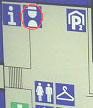
\includegraphics{images/rai_controle.jpg}
\end{center}
\caption{Icoon voor bewaking? (RAI)}
\label{figuur:rai_controle}
\end{figure}


\subsection{AHOY Rotterdam}


\subsubsection{Emoties}

Vrijwel alle onderdelen van de bewegwijzering in AHOY gebruiken een rode tekst en iconen op een witte achtergrond. Dit sluit goed aan bij de uitstraling van het complex. Alles ziet er mooi en zakelijk uit en de leesbaarheid is goed.


\subsubsection{Creativiteit}

Naast de rode tekst is er weinig opvallends te zien op creatief gebied.


\subsubsection{Betekenis}

Er wordt op veel borden naast Nederlandse tekst ook Engelse tekst gebruikt, zodat ook buitenlanders de borden begrijpen. De gebruikte iconen zijn duidelijk en vrij standaard, dus hiervan is de betekenis ook altijd duidelijk.

Richtingen worden aangegeven met pijltjes en als de roltrap of lift gebruikt moet worden wordt dat vermeld. Ook hier geen dubieuze betekenissen.


\subsection{VU Academisch Ziekenhuis Amsterdam}


\subsubsection{Emoties}

Het bewegwijzeringssysteem komt erg goed over, je hebt wel een goed gevoel over de vordering van je actie, want je komt steeds specifiekere richtingaanwijzers tegen. Het komt verder professioneel en zakelijk over. Alleen zijn er ook nog plekken waar er nog afgeweken wordt van het systeem, dat maakt het wat onoverzichtelijker en wat chaotisch. Dit ligt waarschijnlijk aan de nieuwheid van het systeem.


\subsubsection{Creativiteit}

Het systeem zelf is erg zakelijk en niet heel creatief. Wel is het systeem erg duidelijk.


\subsubsection{Betekenis}

De betekenis van de borden is erg duidelijk, wel heb je eerst een korte uitleg nodig bij de informatiebalie.  Verder weet je meteen wel wat er bedoelt wordt met de borden. Het systeem is ook overzichtelijk alleen kan je niet meteen de hele route zien.


\section{Conclusie}

De RAI gebruikt als bewegwijzering borden, iconen en plattegronden. Deze plattegronden zijn situatie gericht, wat naar onze mening een positief punt is. Aanvankelijk hadden we het idee dat dat niet zo zou zijn, maar toen we er gebruik van maakten vonden we het toch wel prettig werken.

Ook vinden we het handig dat in het midden van de hallen vanen hangen met daarop het halnummer zodat je overal in de hal duidelijk kan zien in welke hal je je bevindt.

De plattegronden vinden we niet goed wat betreft de details. Over het algemeen zijn er te veel details, het lijkt af en toe wel een bouwtekening. Maar we missen wel weer een detail: verschil in verdiepingen. De gebruikte iconen op de plattegrond zijn in orde, met als uitzondering het icoon voor kaartcontrole. Het is namelijk niet duidelijk dat het hier om een persoon gaat.

We vinden de RAI niet consistent wat betreft de aanduiding van evenementen. We zien veel tijdelijk objecten en borden. Naar onze mening zou de RAI dit zelf moeten regelen, net zoals dat ook gebeurt in de AHOY. Wat de evenementen binnen de halen ophangen en neerzetten mogen ze zelf weten, maar de bewegwijzering binnen het complex naar de evenementen toe moet de RAI zelf regelen. Dit kan waarschijnlijk het beste met digitale borden.

Verder vinden we het opvallend dat de RAI geen verwijzingen binnen het complex heeft naar toiletten, maar hebben ze alleen iconen op de plattegrond. In het VU ziekenhuis gebeurde dit ook niet (en dat vonden we een groot gemis), maar in de AHOY juist wel. Toch vinden we het niet positief of negatief, er valt namelijk voor beide systemen wat te zeggen. In de RAI zijn veel toiletten en voordat je bij je hal bent aangekomen ben je er waarschijnlijk al 1 of 2 tegengekomen.


\paragraph{Positieve punten}

\begin{itemize}
\item situatie gerichtheid van de plattegronden
\item vanen in de zalen geven goed aan in welke zaal je je bevindt
\end{itemize}


\paragraph{Negatieve punten}

\begin{itemize}
\item betekenis van 1 icoon niet duidelijk
\item plattegrond bevat te veel details
\item plattegrond maakt geen verschil in verdiepingen
\item niet consistent met aanduiding evenementen: veel tijdelijke objecten en borden
\item RAI regelt de bewegwijzering binnen het comlex naar het evenement toe niet zelf
\end{itemize}


\paragraph{Overige punten}

\begin{itemize}
\item toiletten worden alleen aangegeven op de plattegrond, er zijn geen pijlen in de gangen die ernaar wijzen
\end{itemize}
